\section{Gravitational Time Dilation}

\label{gravity_time_lab}
\makelabheader %(Space for student name, etc., defined in master.tex)

\bigskip

\textbf{Activity 1: The Doppler Effect}

The postulate of relativity tells us that the speed of light $c$ is the same in all reference frames, and is not affected by the speed of the source or the receiver.  But the relative velocity of the source and the receiver \textit{does} affect the wavelength and frequency of the light.  This is known as the relativistic Doppler effect.  (A similar, non-relativistic Doppler effect occurs with sound: you hear the pitch of a siren or horn change as a car speeds by you, higher as the car approaches you and lower as the car moves away.)

\begin{center}
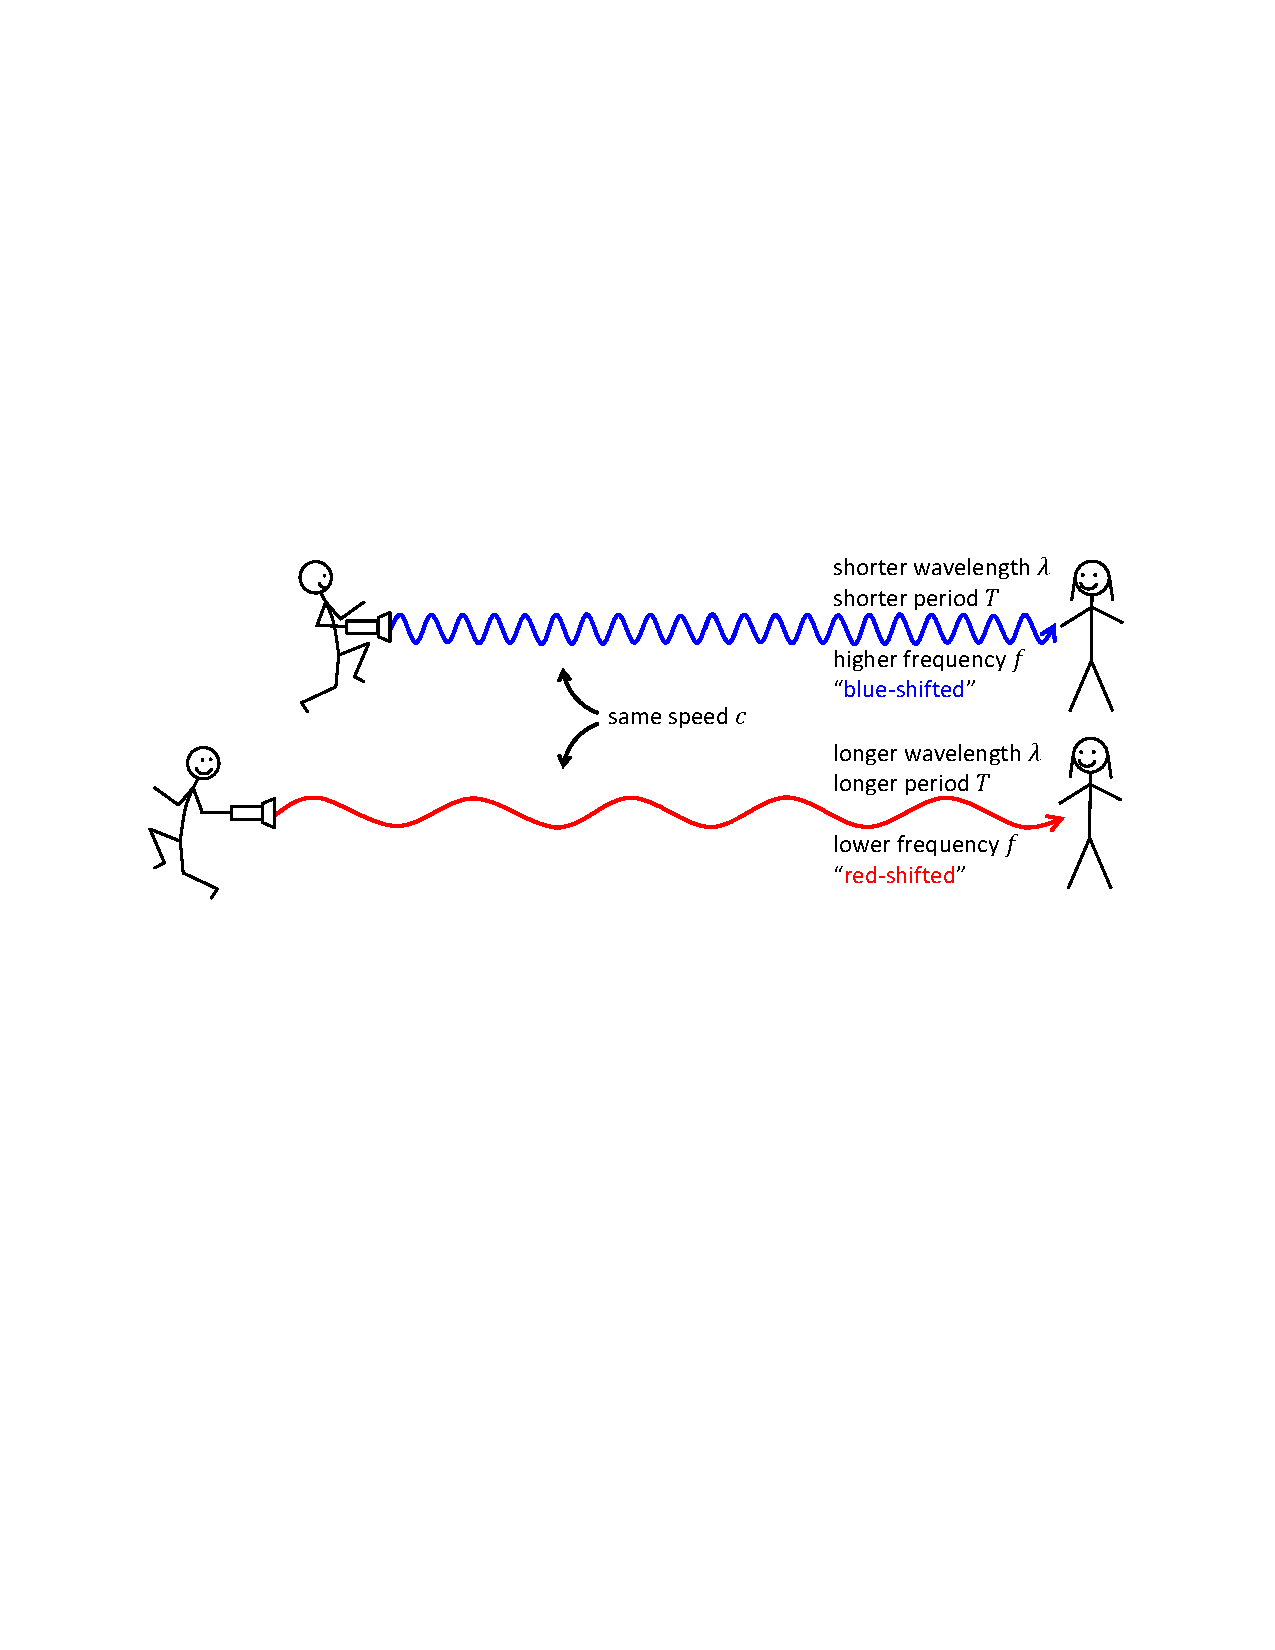
\includegraphics[width=0.75\textwidth]{gravity_time/red_shift_blue_shift.pdf}
\index{color page}
\end{center}

If the source and receiver are approaching each other, the wavefronts are compressed together, shortening the light's wavelength $\lambda$ and the time $\Delta t$ between wave fronts, also known as the period $T$.  This shifts the color of visible light towards the blue end of the spectrum, and we say the light is ``blue-shifted.''  A source and receiver receding away from each other causes the opposite effect, called a ``redshift.''

To examine this effect quantitatively, let's suppose
your friend (the ``source'') is shining a flashlight at you while running towards you at a very fast speed $v$.  The figure below shows the situation as drawn in your reference frame.  The first wavefront is emitted at time $t=0$.

\begin{center}
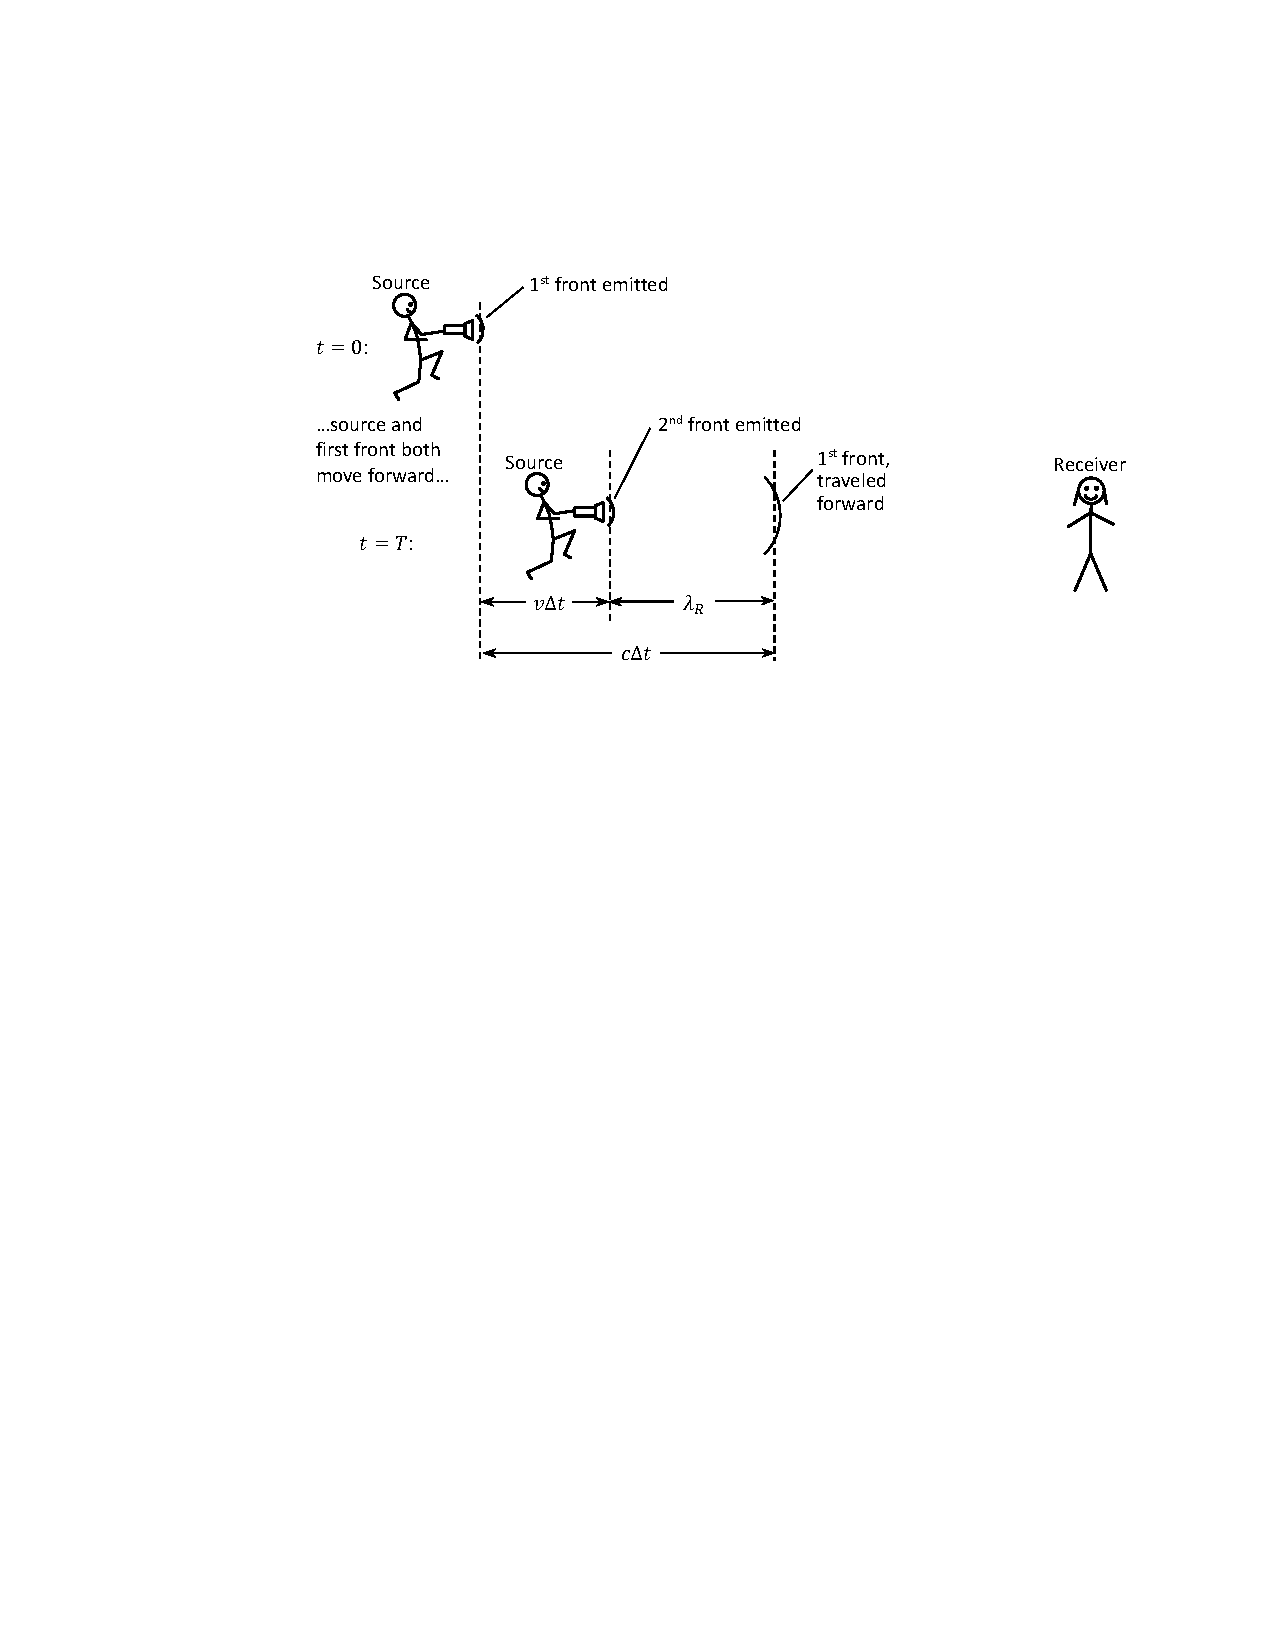
\includegraphics[width=0.75\textwidth]{relativistic_doppler/relativistic_front_motion.pdf}
\end{center}

\begin{enumerate}[labparts]
\item After one period $\Delta t_S=T$, the first wavefront emitted has traveled a distance $c\Delta t_S$, and the source has traveled a distance $v\Delta t_S$.  What is the distance $\lambda_R$ between wavefronts seen by the receiver?  (Answer in terms of $v$, $c$, and $\Delta t_S$.)
\answerspace{0.5in}

\item What is the time $\Delta t_R$ that you measure between when the first wavefront reaches you and when the second wavefront reaches you?  That is, how long does it take the second wavefront to travel a distance $\lambda_R$?
(Answer in terms of $c$ and $\lambda_R$.)
\answerspace{0.5in}

\item Combining your previous two answers, what is the time $\Delta t_R$ that you measure between when the first wavefront reaches you and when the second wavefront reaches you, in terms of $c$, $v$, and $\Delta t_S$?
\answerspace{0.5in}

\item Suppose instead that your friend stands still, and you run towards your friend at the same speed $v$.  Based on the postulate of relativity, would your answer to the previous part be any different?
\answerspace{0.5in}

\item For tidiness, we sometimes express the speed of an object using $\beta \equiv v/c$, where $\beta$ is the Greek letter ``beta.''  (There's no good name for $\beta$, since it's really just the velocity $v$ in units of $c$, so we just call it ``beta.'')  Express your result for $\Delta t_R$ in terms of $\Delta t_S$ and $\beta$.\footnote{
You may have noticed that we've cheated a little bit in this activity by ignoring any time dilation due to the source's velocity.  In fact, only the source would measure the proper time $\Delta t_0$ between the first and second wavefronts being emitted; the receiver would see that time dilated by a factor of $\gamma = \left(1-\beta^2\right)^{-1/2}$.  Taking this into account, the correct expression would be 
$\Delta t_R = \sqrt{\frac{1 - \beta}{1+\beta}}\Delta t_S$, or
$f_R = \sqrt{\frac{1 + \beta}{1-\beta}}f_S$.  For low speeds $v << c$, these reduce to the simpler form you just derived, $\Delta t_R \approx (1 - \beta)\Delta t_S$.
}
\answerspace{0.5in}

You noted before that it doesn't matter whether it's you or your friend who is running; what matters is simply whether the two of you are approaching each other or receding away from each other.  This leads to a funny sign convention.  In the expression $\Delta t_R = (1 - \beta)\Delta t_S$, we use a positive number for $\beta$ if the source and receiver are approaching each other, and a negative number for $\beta$ if the source and receiver are receding from each other:  
\begin{align*}
\textrm{positive } \beta &\Longrightarrow \textrm{motion towards each other (``approaching'')} \\
\textrm{negative } \beta &\Longrightarrow \textrm{motion away from each other (``receding'')}. 
\end{align*}
This means that we might use a positive $\beta$ even if the receiver is moving in the $-x$ direction.
\end{enumerate}

\textbf{Activity 2: The Relativistic Doppler Effect in an Accelerating Rocket}

Suppose you are in a rocket ship in interstellar space, far away from any stars or planets.  (See the figure on the following page) Although there is essentially no gravity, your rocket is accelerating at $a=g=9.8$~m/s$^2$ to make you feel at home.  You set up an experiment with a light source at the back end of the rocket and you at the front end, a distance $H$ away from the source.  The source emits light with a known frequency and wavelength, and a period $T$ between wavefronts of $T=\Delta t_S$.

\begin{enumerate}[labparts]
\item How long is the time $\Delta t_{\rm trip}$ does it take the light to travel the distance $\Delta x = H$ from the back of the rocket to the front of the rocket?  (Answer in terms of $c$ and $H$.)
\answerspace{0.5in}

Although you and the source are always going exactly the same speed at any time, we still need to account for the relativistic Doppler effect, because the rocket is accelerating.  By the time the light reaches you, your speed is different from what the speed of the source was when the light was emitted.

\begin{minipage}{0.6\textwidth}

\item Does the acceleration of the rocket cause the light reaching you to be \textit{red-shifted} or \textit{blue-shifted}?
\answerspace{0.5in}

\item By how much $\Delta v$ has your speed increased during the time $\Delta t_{\rm trip}$ it took for the light to reach you? Answer in terms of $g$ and $\Delta t_{\rm trip}$.  (Hint: $v = \Delta x / \Delta t$, and $a = \Delta v / \Delta t$.)
\answerspace{0.5in}


\item Now consider the period $T = \Delta t_S$ of the light source, which is the time between the emission of two wave fronts.  If you measure the time between wavefronts when they reach you, is your time $\Delta t_R$ \textit{longer} or \textit{shorter} than $\Delta t_S$?
\answerspace{0.5in}


\item Write your time between wavefronts $\Delta t_R$ in terms of $\Delta t_S$ and $\beta$, where $\beta$ is the relative speed between you (when you receive the light) and the source (when it emits the light).
\answerspace{0.5in}
\end{minipage}
\begin{minipage}{0.39\textwidth}
\hspace{\fill}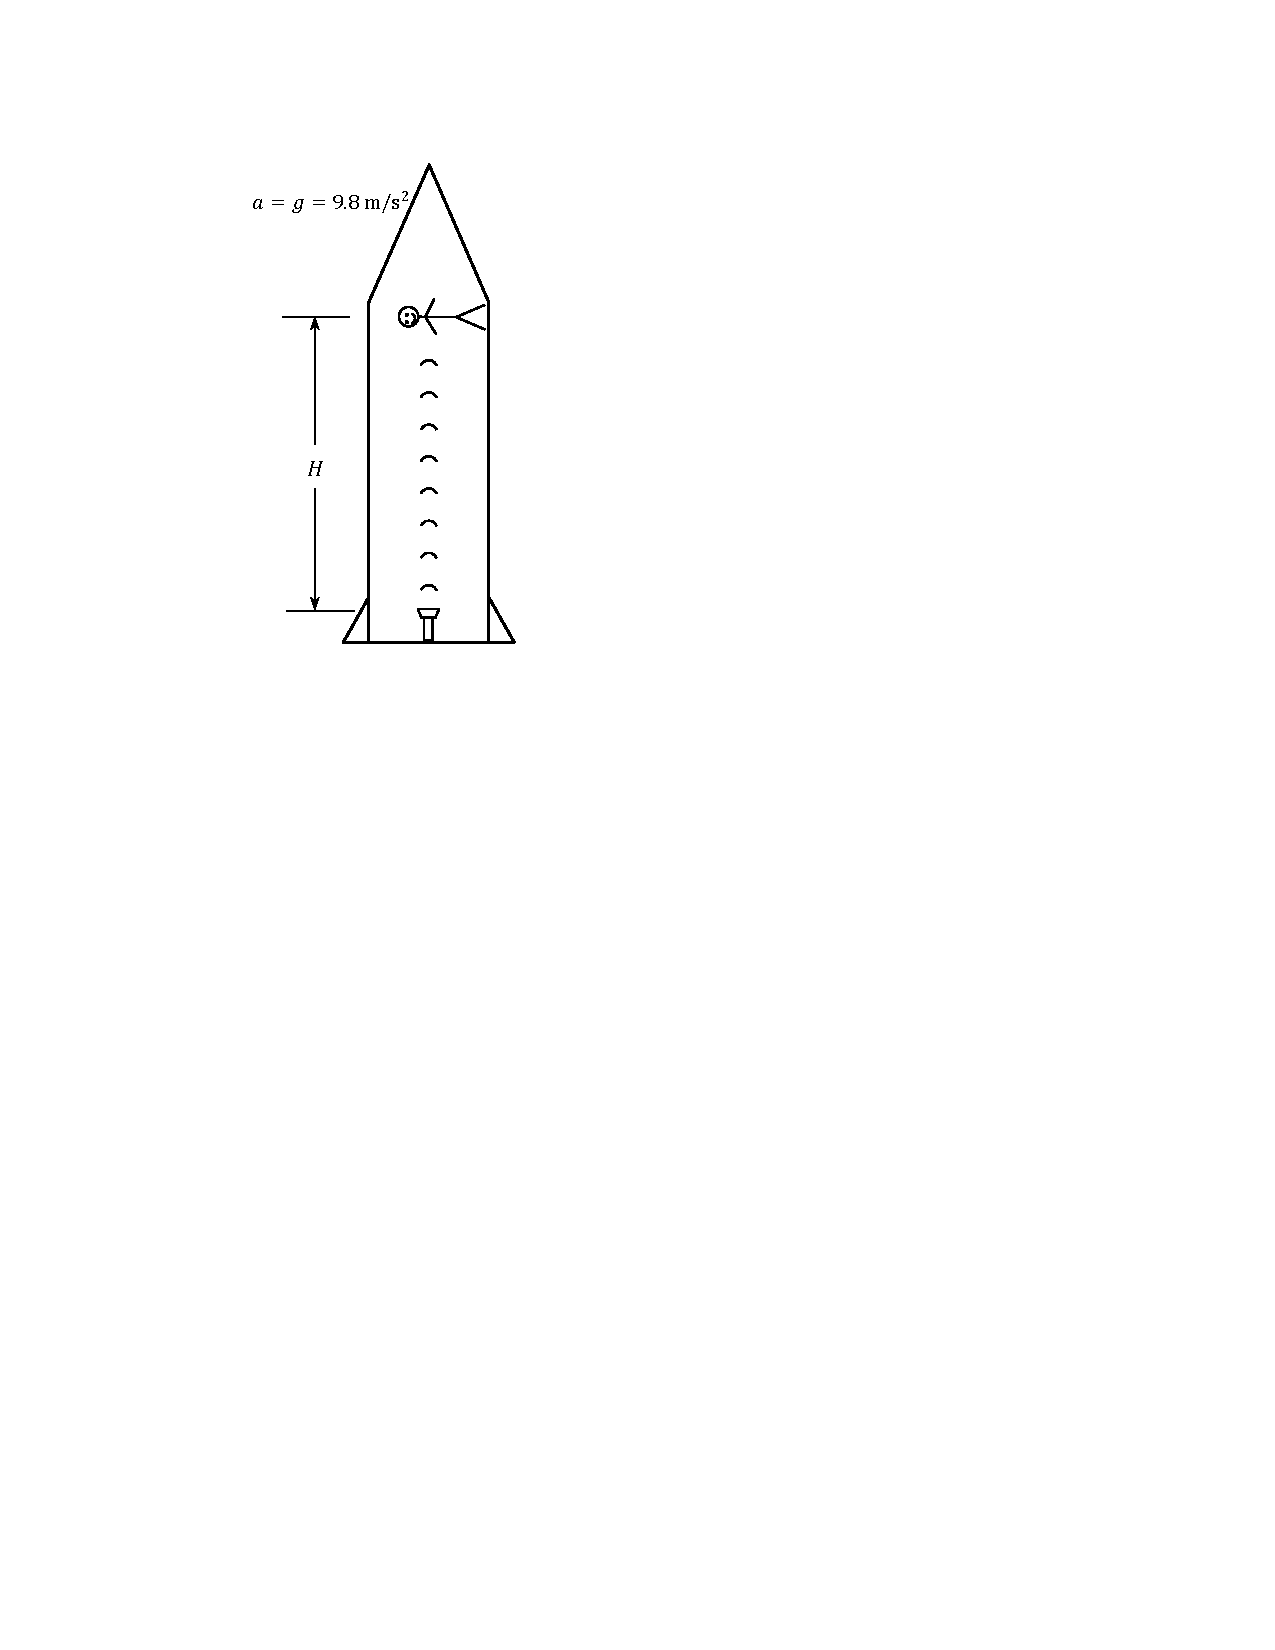
\includegraphics{gravity_time/accelerating_rocket.pdf}
\end{minipage}

\item What is the value of $\beta$ in terms of $g$, $\Delta t_{\rm trip}$, and $c$?  Be careful with your signs here: should the value of $\beta$ be \textit{positive} or \textit{negative}?
\answerspace{0.5in}

\item Write your time between wavefronts $\Delta t_R$ in terms of $\Delta t_S$, $g$, $H$, and $c$.  Again, be careful with your signs: your $\Delta t_R$ should be greater than $\Delta t_S$, right?
\answerspace{0.5in}

\end{enumerate}